\documentclass[11pt,a4paper]{article}
\usepackage[utf8]{inputenc}
\usepackage[T1]{fontenc}
\usepackage[margin=2.5cm]{geometry}
\usepackage{parskip}
\usepackage{setspace}
\usepackage{graphicx}
\usepackage{booktabs}
\usepackage{hyperref}
\usepackage{xcolor}
\usepackage{enumitem}
\usepackage{listings}
\usepackage[most]{tcolorbox}

% ---------------- Listings (Python) ----------------
\lstdefinestyle{pythonstyle}{
    language=Python,
    basicstyle=\ttfamily\small,
    showstringspaces=false,
    breaklines=true,
    keywordstyle=\color{blue!70!black},
    stringstyle=\color{teal!60!black},
    commentstyle=\color{gray!70},
    frame=single,
    numbers=left,
    numberstyle=\tiny\color{gray},
    stepnumber=1,
    numbersep=8pt,
    columns=fullflexible
}
\lstset{style=pythonstyle}

% ---------------- Tcolorbox for Tips/Notes ----------------
\tcbset{
    colback=gray!3,
    colframe=gray!50,
    boxrule=0.4pt,
    arc=2mm,
    left=6pt,right=6pt,top=6pt,bottom=6pt
}

\title{\textbf{Analisis Korelasi Data Bike Sharing dan Identifikasi Variabel Independen}}
\author{Rafa Al Razzak \\ \texttt{0110224155@student.nurulfikri.ac.id}}

\begin{document}
    \maketitle
    \onehalfspacing

    \begin{abstract}
        Dokumen ini menyajikan analisis korelasi terhadap dataset bike sharing yang berisi informasi penyewaan sepeda harian.
        \hspace{1cm}Analisis dimulai dengan memuat data, melakukan preprocessing dengan menghapus kolom tanggal, kemudian menganalisis korelasi antar variabel menggunakan heatmap.
        \hspace{1cm}Dataset memiliki variabel dependen \texttt{cnt} (total penyewaan sepeda) dan berbagai variabel independen seperti kondisi cuaca, musim, dan faktor temporal.
        \hspace{1cm}Tujuan analisis adalah mengidentifikasi faktor-faktor yang paling berpengaruh terhadap jumlah penyewaan sepeda untuk persiapan pemodelan prediktif.
    \end{abstract}

    \vspace{-1mm}


    \section{Memuat Dataset}
    Memuat dataset bike sharing yang berisi informasi penyewaan sepeda harian.
    \begin{lstlisting}[language=Python]
import pandas as pd

df = pd.read_csv("../DATA/day.csv")
df.head()
    \end{lstlisting}

    \begin{figure}[h]
        \centering
        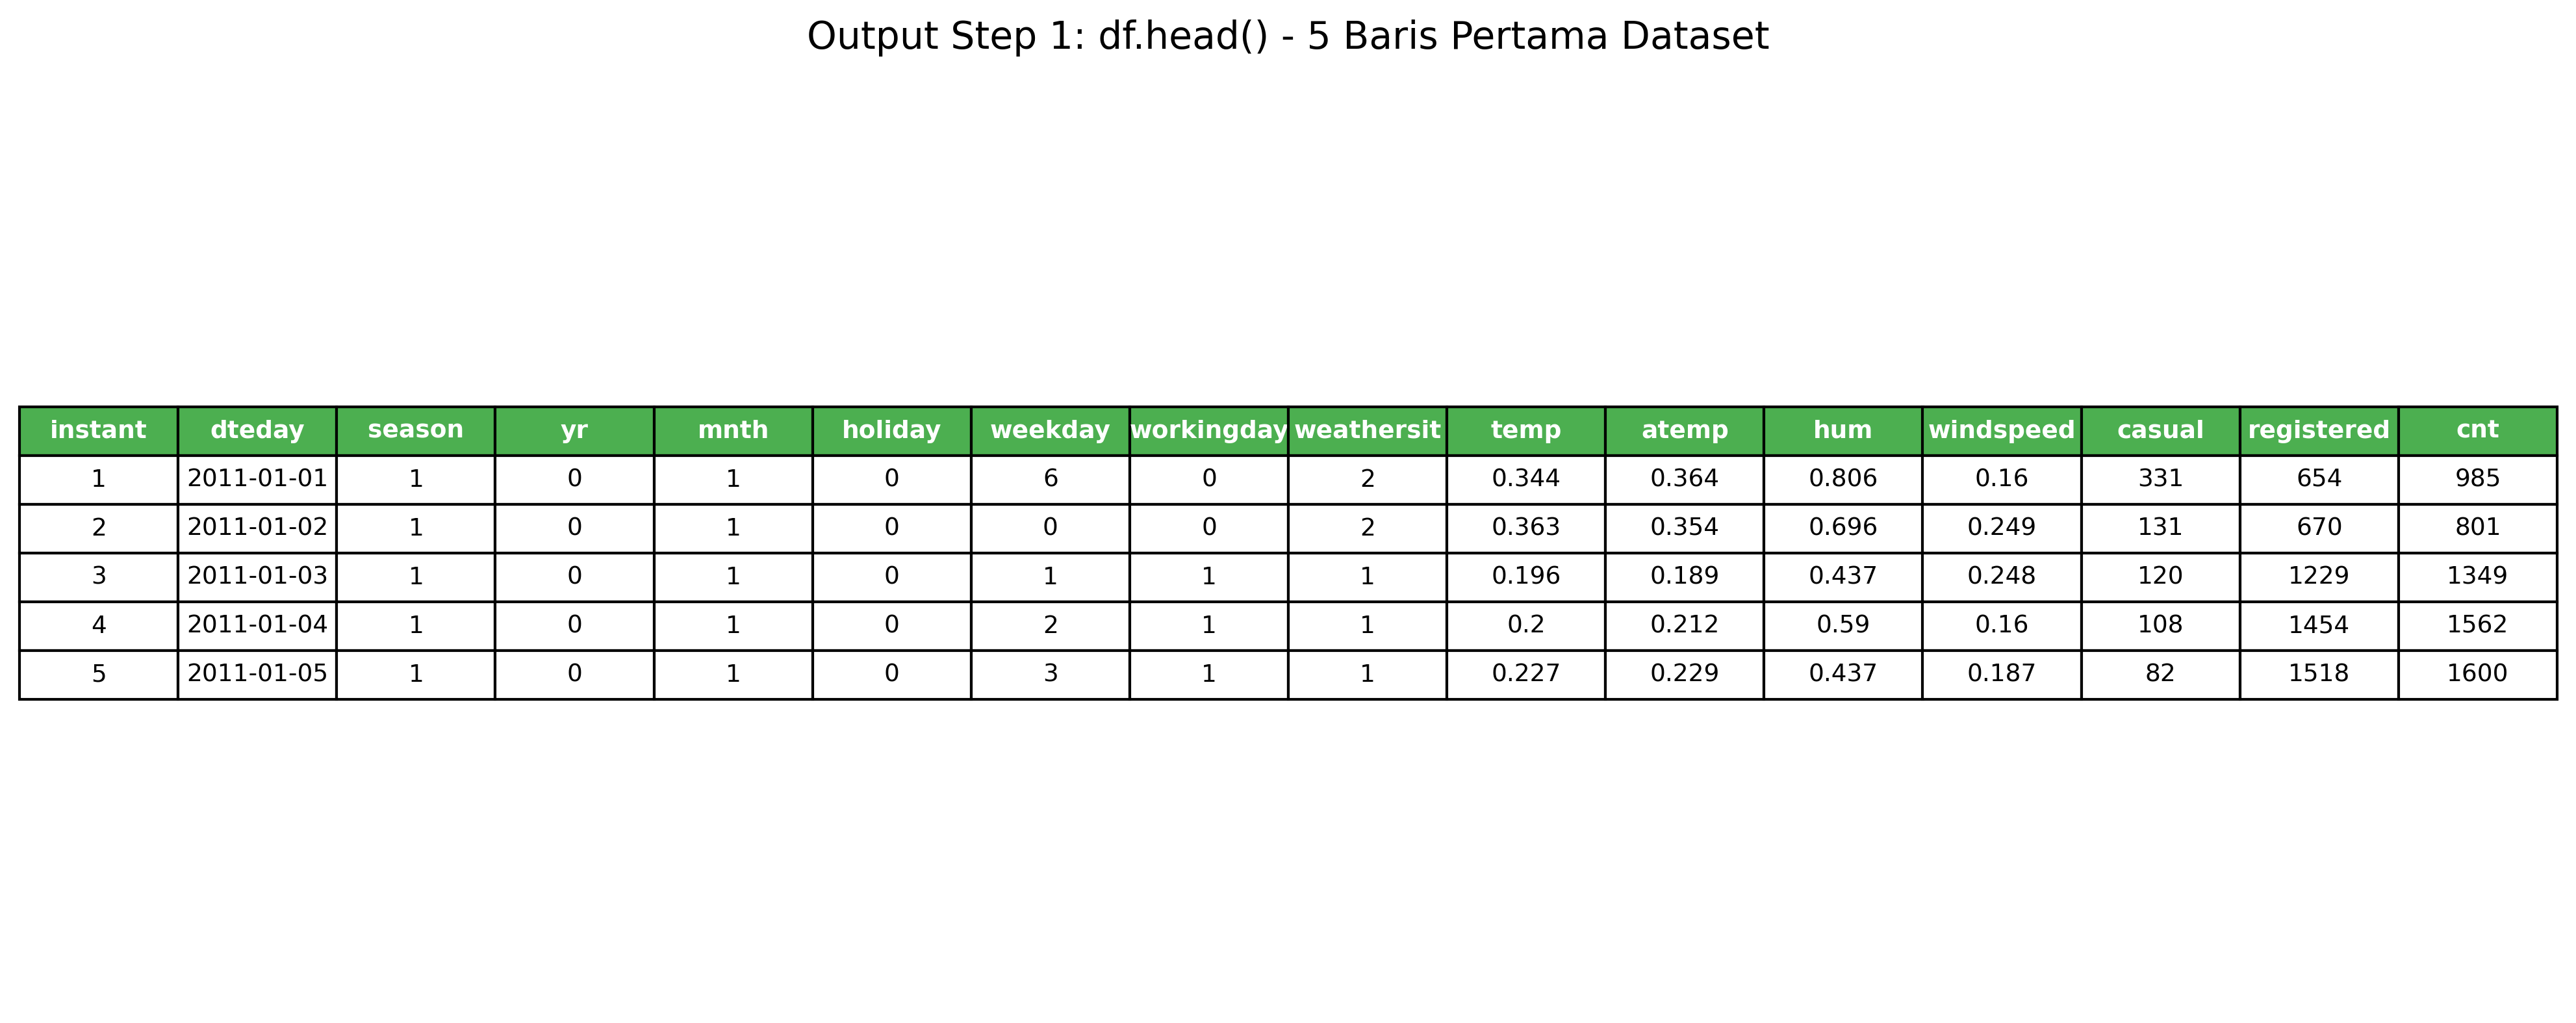
\includegraphics[width=1.0\textwidth]{./OUTPUT/step1_data_head.png}
        \caption{Output Step 1: Hasil dari df.head() - Menampilkan 5 Baris Pertama Dataset}
        \label{fig:data_head}
    \end{figure}

    \begin{tcolorbox}
        \textbf{Dataset:} Berisi 16 kolom dengan data penyewaan sepeda dari 2011-2012, termasuk informasi cuaca, musim, dan temporal.
        \hspace{1cm}Dataset memiliki 731 baris data harian.
    \end{tcolorbox}


    \section{Preprocessing Data}
    Menghapus kolom yang tidak diperlukan untuk analisis korelasi.
    \begin{lstlisting}[language=Python]
df_processed = (
    df
    .drop(columns=["dteday"])
).copy()
    \end{lstlisting}
    \begin{tcolorbox}
        \textbf{Alasan:} Kolom \texttt{dteday} (tanggal) dihapus karena tidak diperlukan dalam analisis korelasi numerik.
        \hspace{1cm}Data yang diproses siap untuk perhitungan korelasi.
    \end{tcolorbox}


    \section{Menghitung Matriks Korelasi}
    Menghitung matriks korelasi untuk melihat hubungan antar variabel numerik.
    \begin{lstlisting}[language=Python]
corr_matrix = df_processed.corr()
corr_matrix.head()
    \end{lstlisting}

    \begin{figure}[h]
        \centering
        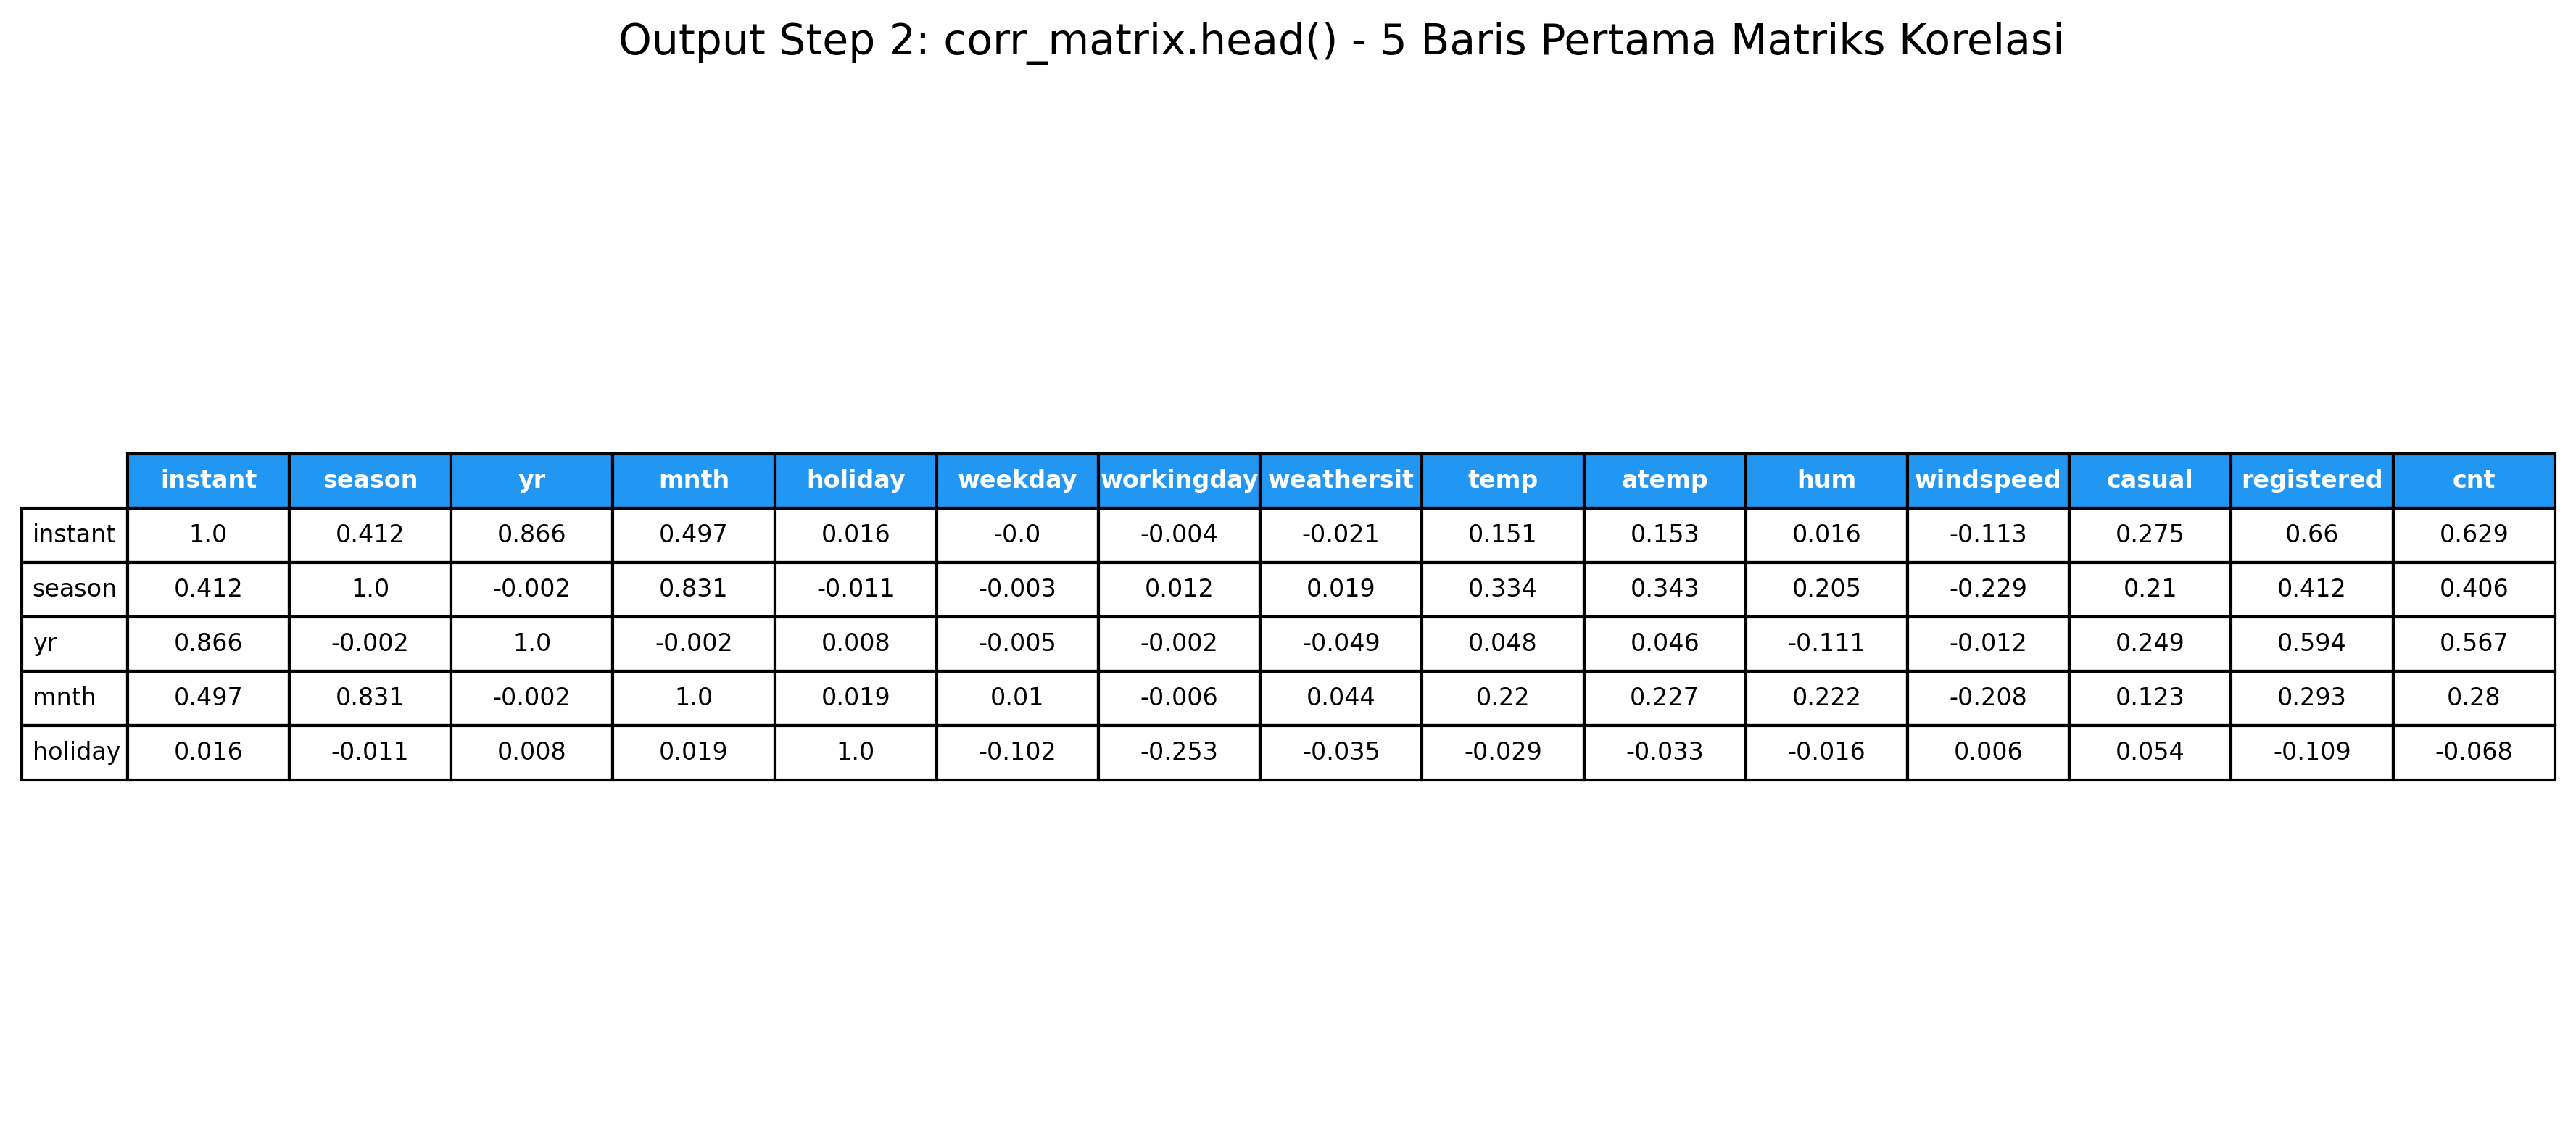
\includegraphics[width=1.0\textwidth]{./OUTPUT/step2_correlation_head.png}
        \caption{Output Step 2: Hasil dari corr\_matrix.head() - Matriks Korelasi 5 Baris Pertama}
        \label{fig:corr_head}
    \end{figure}

    \begin{tcolorbox}
        \textbf{Interpretasi:} Matriks korelasi menunjukkan nilai korelasi Pearson antara -1 hingga 1.
        \hspace{1cm}Nilai mendekati 1 menunjukkan korelasi positif kuat, nilai mendekati -1 menunjukkan korelasi negatif kuat, dan nilai mendekati 0 menunjukkan tidak ada korelasi.
    \end{tcolorbox}


    \section{Visualisasi Heatmap Korelasi}
    Memvisualisasikan matriks korelasi menggunakan heatmap untuk analisis yang lebih mudah.
    \begin{lstlisting}[language=Python]
import matplotlib.pyplot as plt
import seaborn as sns

plt.figure(figsize=(8, 6))
sns.heatmap(corr_matrix,
           annot=True, cmap="coolwarm", fmt=".2f")
plt.title("Korelasi Variabel")
plt.show()
    \end{lstlisting}

    \begin{figure}[h]
        \centering
        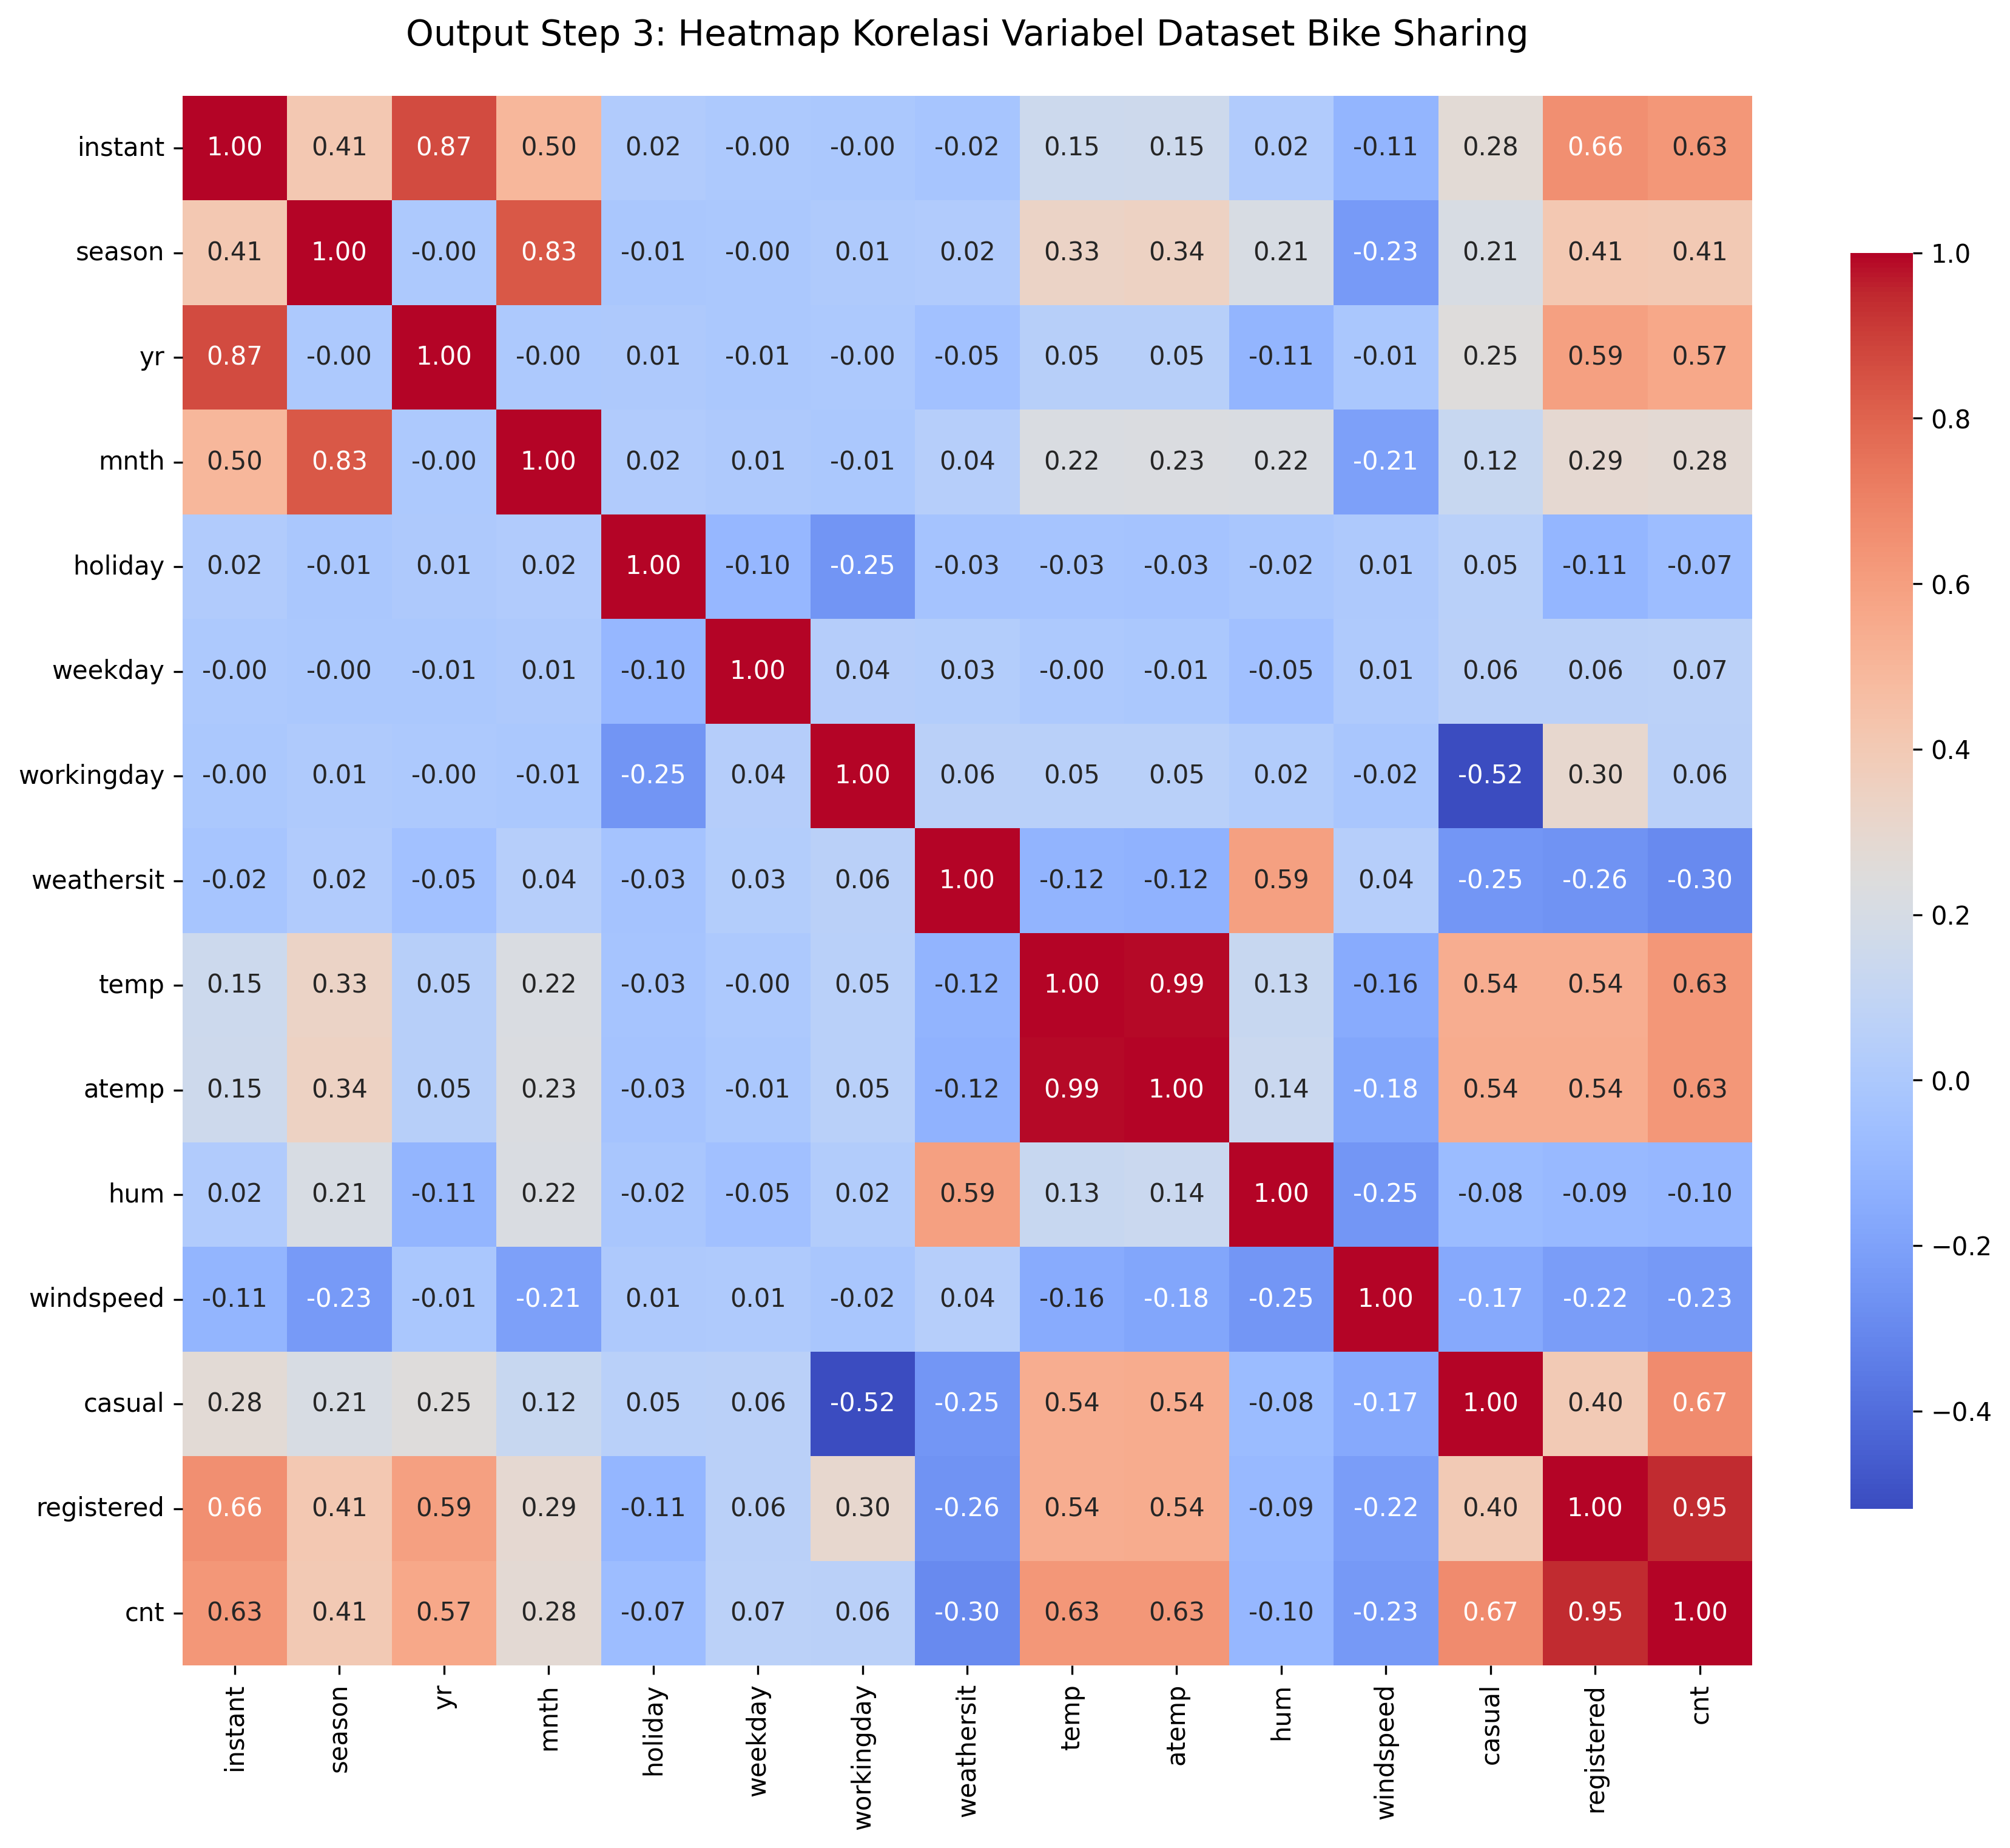
\includegraphics[width=1.0\textwidth]{./OUTPUT/step3_heatmap.png}
        \caption{Output Step 3: Heatmap Korelasi Lengkap Antar Semua Variabel Dataset Bike Sharing}
        \label{fig:heatmap_full}
    \end{figure}

    \begin{tcolorbox}
        \textbf{Interpretasi Heatmap:} Warna merah menunjukkan korelasi positif yang kuat, warna biru menunjukkan korelasi negatif, dan warna putih menunjukkan tidak ada korelasi.
        \hspace{1cm}Setiap sel menampilkan nilai korelasi dengan 2 desimal untuk analisis yang detail.
    \end{tcolorbox}


    \section{Interpretasi Hasil Korelasi}
    Dari heatmap korelasi, dapat diidentifikasi:

    \begin{enumerate}
        \item \textbf{Korelasi Positif Kuat}: Variabel yang meningkatkan jumlah penyewaan
        \item \textbf{Korelasi Negatif}: Variabel yang menurunkan jumlah penyewaan
        \item \textbf{Korelasi Lemah}: Variabel dengan pengaruh minimal
    \end{enumerate}


    \section{Kesimpulan}
    Analisis korelasi menggunakan heatmap memberikan wawasan penting untuk:
    \begin{itemize}
        \item \textbf{Pemilihan fitur}: Mengidentifikasi variabel independen yang paling berpengaruh terhadap \texttt{cnt}
        \item \textbf{Menghindari multikolinearitas}: Tidak menggunakan variabel yang berkorelasi tinggi secara bersamaan
        \item \textbf{Pemahaman bisnis}: Memahami faktor cuaca, musim, dan temporal yang mempengaruhi penyewaan sepeda
        \item \textbf{Persiapan modeling}: Menyiapkan dataset untuk tahap pemodelan machine learning selanjutnya
    \end{itemize}

    Dataset ini sangat cocok untuk membangun model regresi prediktif dengan variabel target \texttt{cnt} dan berbagai variabel independen yang telah diidentifikasi dari analisis korelasi.


    \section{Kode Sumber}

    \subsection{GitHub Repository}
    Kode lengkap dari analisis ini dapat ditemukan di GitHub repository berikut:

    \begin{tcolorbox}[colback=blue!5,colframe=blue!50]
        \textbf{Link GitHub:} \\
        \href{https://github.com/sttnf/machine-learning/tree/main/PERTEMUAN\%203/TUGAS/NOTEBOOKS/main.ipynb}{\texttt{PERTEMUAN 3/TUGAS/NOTEBOOKS/main.ipynb}}

    \end{tcolorbox}

\end{document}
